\subsection{Methodology}
This project lends itself to being suitable for an agile development methodology, given that it is small with a single inexperienced developer, requirements and time constraints may change, and having frequent builds with new progress ensures that a functioning product will exist by the end. Sprints will range from 1-3 weeks long depending on the difficulty of the task being worked on in that sprint, and the time available to work on the project during the sprint. 

To ensure that the software meets the requirements set out by the customer, the objectives settled on have been based on a similar set of requests from the customer, and communication with the customer will continue through the project. Various builds may be provided in order to get feedback that can be implemented in the next sprint.

Supervisor meetings will be arranged only when needed, when progress has been made, or extended discussion of ideas is required.

All project code and documents will be stored in a GitHub repository with CI\textbackslash CD configured in GitHub Actions to ensure the latest production version compiles. Online hosted version control ensures that access to the codebase and documents is simple and always available, and that mistakes can be reverted if needed. CI\textbackslash CD ensures that a testable version of the project is available at all times so feedback can be gained more often and on a recent version and no extra effort will be required to create a functioning prototype for the presentation.

\subsection{Timetable}
Taking into account deadlines for both this project and for the coursework of other modules, an initial timetable includes all essential parts of the system in term 1, with the most important features implemented by the due date of the progress report. All high priority features should be implemented by the start of the winter holidays, and additional features will follow during the winter holidays and term 2. Task dependencies are mostly linear with each task requiring the previous one to be completed, or only makes sense to be completed after the previous one because the tasks are planned to be undertaken in order of importance. Each task will include a substantial amount of time spent researching how to perform it, such as identifying suitable technologies, APIs, or data required to implement a feature. It is expected that this timetable will be accurate only in the short term, given that projects of this scale are very likely to encounter delays caused by unforeseen issues, hence an up to date version of the timetable will be maintained. Some possible delay causing events are clashes with the completing of coursework from other modules, so a longer period of time has been allocated to tasks which should be performed during these periods, which also gives time for breaks from the project.

% Gantt image
\begin{figure}[H]
    \centering
	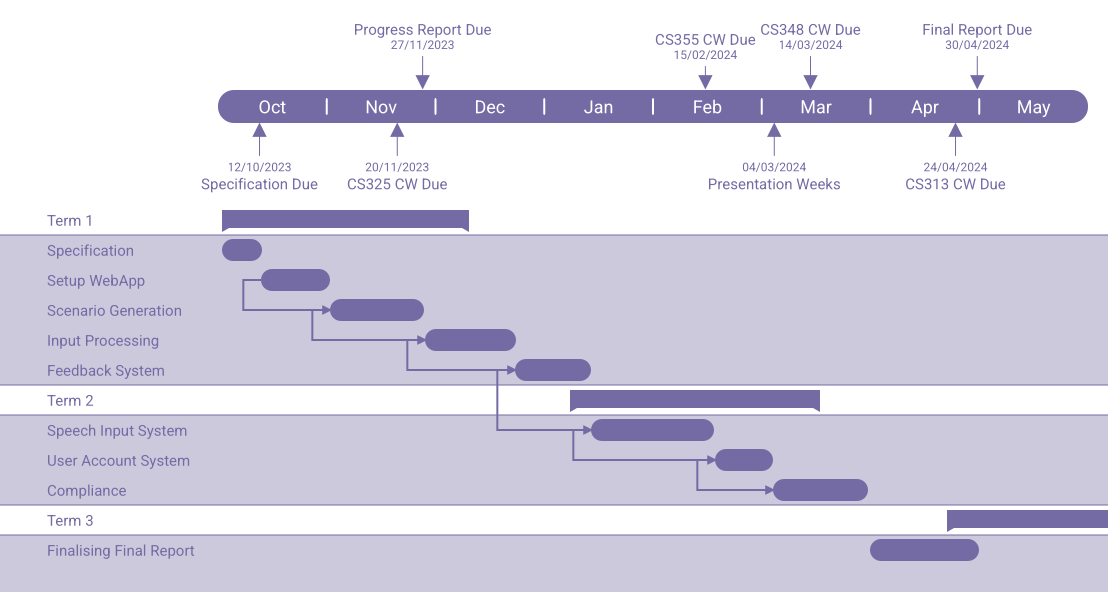
\includegraphics[scale = 0.42]{../document-resources/images/initial-gantt.png}
    \label{initialgantt}
    \caption{Proposed project timeline}
\end{figure}

\subsection{Risk Assessment}
The risks involved in this project are primarily related to the people and technologies required to build it.
The technology risks include access to the APIs that will be relied upon to obtain data which I cannot feasibly obtain myself within the scope of the project.
At any time the APIs could be changed or removed which would require a change in the project scope, but can be somewhat mitigated by keeping features modular, so that they can be removed or replaced with minimal impact on the rest of the system.
The Google Maps API is free for \$200 worth of transactions per month, which should be sufficient for the project. However, it is possible that this limit be reached, which would require reconsidering the use of the API, but other similar APIs exist such as the Bing Maps API which offers limited educational usage.

Given that implementing even pre-trained machine learning models can be difficult, the speech-to-text conversion may need to be done by an external API if time constraints require it. Various such APIs exist with free tiers of access suitable for the project such as Google Speech API. A text-to-speech API will not be required as modern browsers include text-to-speech capabilities.

\subsection{Resources \& Technologies}
\begin{itemize}
    \item GitHub Repositories, Actions. Using a version control system reduces development issues and improves code availability.
    \item Languages: Javascript, HTML, CSS. Performance will not be a major requirement as the expected user count is low for the system, hence Javascript is suitable as it fields countless libraries and provides a good developer experience.
    \item Libraries: Whisper for Speech to Text conversion, SvelteKit for simplifying web app development.
    \item APIs: Google Maps API for aerial map data, Google Speech API (if own implementation proves infeasible).
    \item Customer
    \item Documents: CAP413 RT manual, EGAST Phraseology Guide, 
\end{itemize}

\subsection{Legal, Social, Ethical, Professional Issues and Concerns}
Given that the target users of the system will mainly be trainee pilots, it is paramount that the information taught by the system follows the guidelines set by the UK Civil Aviation Agency (CAA), given that incorrect or insufficient teaching has shown itself to be a factor in the causes of multiple aircraft incidents in the last two decades. If the software is to be used for training, care must be taken to insure that it reflects correct teaching of radio communications as set out in the CAP 413: Radiotelephony Manual \cite{CAP413}. This could be resolved by working with trained flight instructors and examiners to validate the system's information, and the inclusion of a notice to all users that the software should only be used alongside lessons from a qualified instructor.